\subsection{Polare stereographische Projektion}
\label{sec:polstere}
Die polare stereographische  Projektion ist eine stereographische Projektion die einen der beiden Pole als Kartenzentrum hat.\\
\begin{figure}[hbtp]
\centering
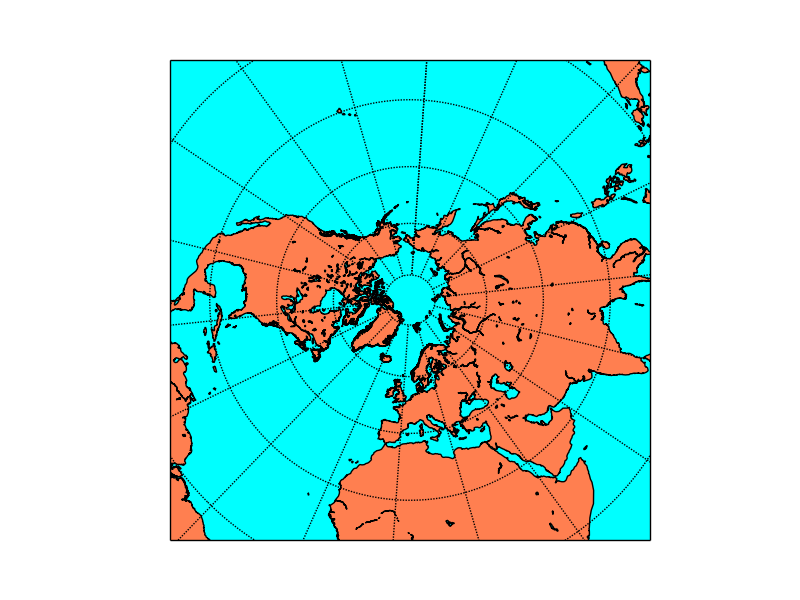
\includegraphics[scale=0.5,origin=c]{/Users/student/seminar/Kartendarstellungen/seminar/npstere} \\
\caption{Nordpol}
\end{figure}
\begin{figure}[hbtp]
\centering
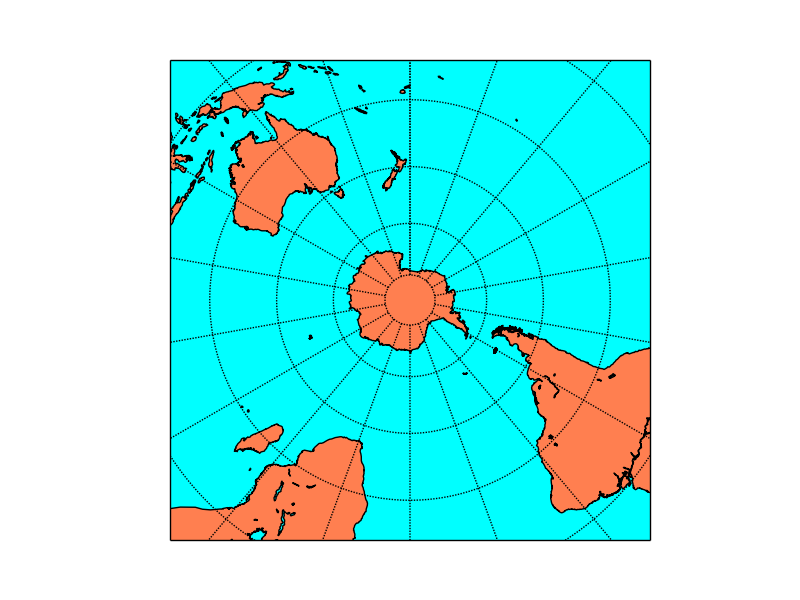
\includegraphics[scale=0.5,origin=c]{/Users/student/seminar/Kartendarstellungen/seminar/spstere} 
\caption{Südpol}
\end{figure}\newpage 
\subsection{Polare azimutale Lambertprojektion}
\label{sec:pollam}
Die polare  azimutale Lambertprojektion hat ebenfalls einfach nur einen Pol als Kartenzentrum.\\
\begin{figure}[hbtp]
\centering
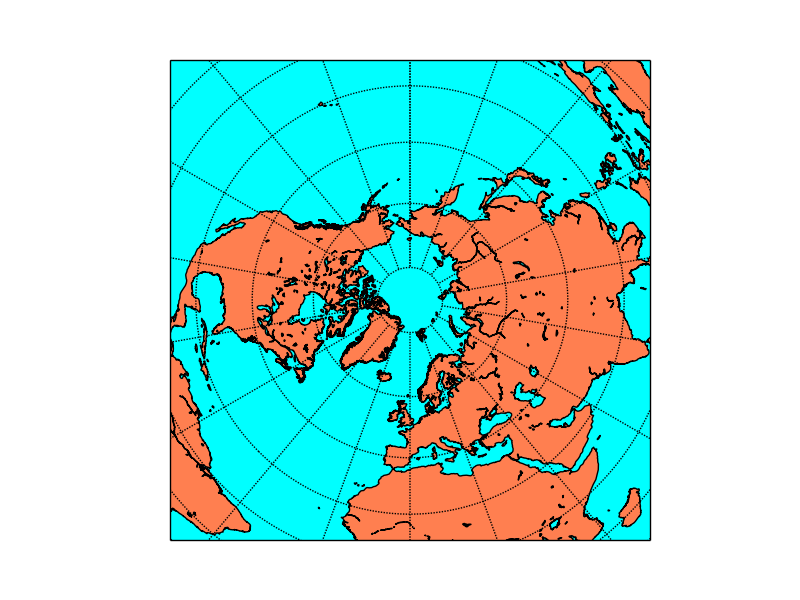
\includegraphics[scale=0.5,origin=c]{/Users/student/seminar/Kartendarstellungen/seminar/nplaea}\\
\caption{Nordpol}
\end{figure}
\begin{figure}[hbtp]
\centering
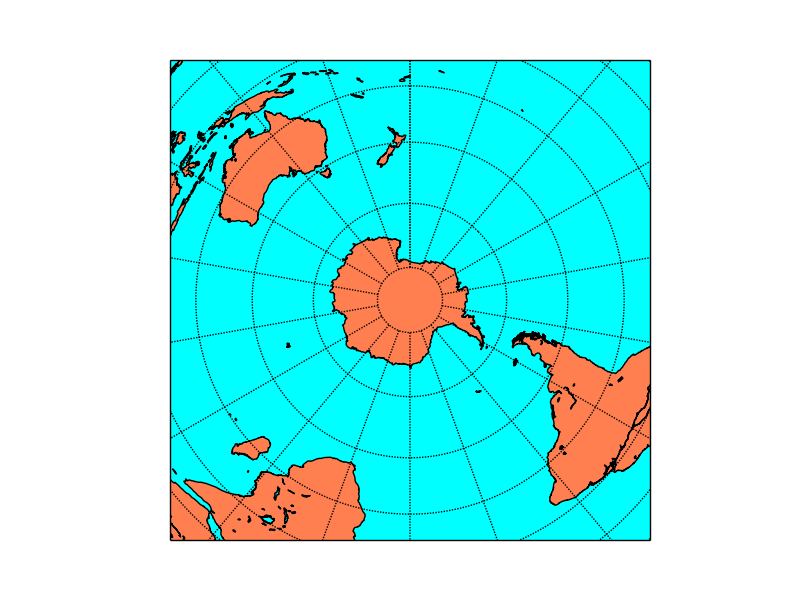
\includegraphics[scale=0.5,origin=c]{/Users/student/seminar/Kartendarstellungen/seminar/splaea} 
\caption{Südpol}
\end{figure}\newpage 
\subsection{Polare azimuthale äquidistante Projektion}
\label{sec:polaequi}
Diese Projektion hat ebenfalls einfach einen Pol als Mittelpunkt. \\
\begin{figure}[hbtp]
\centering
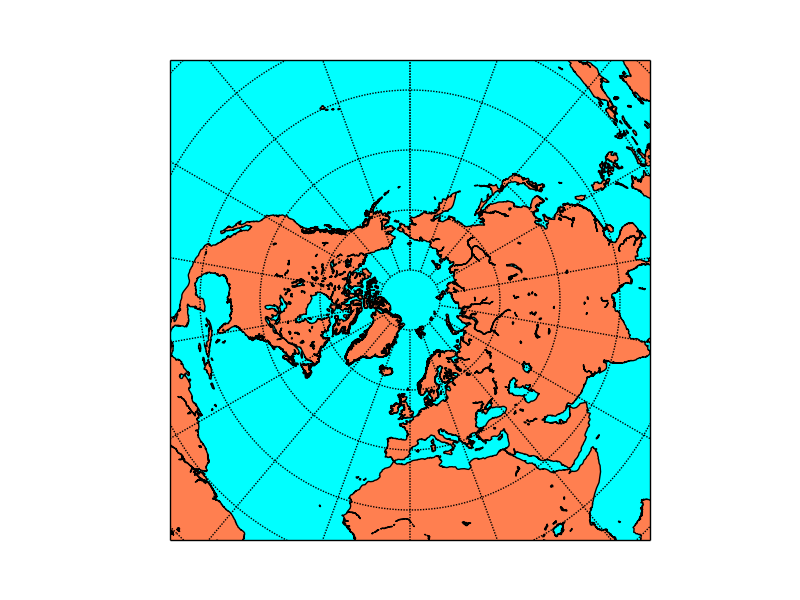
\includegraphics[scale=0.5,origin=c]{/Users/student/seminar/Kartendarstellungen/seminar/npaeqd} \\
\caption{Nordpol}
\end{figure}
\begin{figure}[hbtp]
\centering
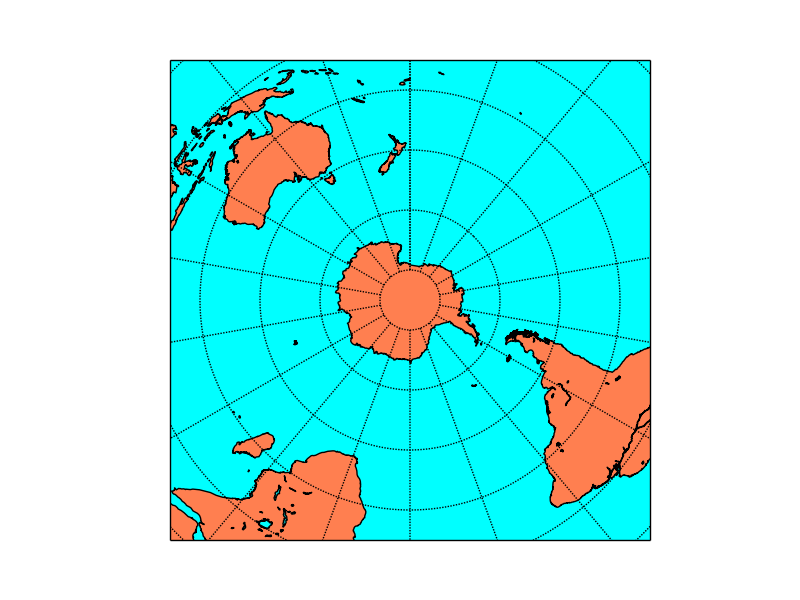
\includegraphics[scale=0.5,origin=c]{/Users/student/seminar/Kartendarstellungen/seminar/spaeqd} \caption{Südpol}
\end{figure}\newpage 
